\subsection{Programa final Unity PRO}

A partir del programa utilizado para los primeros registros, se realizó modificaciones necesarias para borrar y agregar variables que se creyeron necesarias a la hora de implementar el proyecto.


\subsubsection{Direcciones utilizadas}
\fcolorbox{red}{yellow}{Las direcciones utilizadas para unity + ifix ponerlo despues de SCADA?}


\subsection{Adquisición de datos}
Para realizar la estimación de la planta del sistema se utilizó el protocolo OPC en conjunto con Matlab. Por medio de OFS (OPC Factory Server, software de Schneider), se procedió a crear y configurar un servidor con la dirección correspondiente y se seleccionó el programa realizado en UnityPro donde se encontraban las variables necesarias (Figura \ref{fig:opc1}).

\begin{figure}[htbp]
	\centering
	\subfigure[]{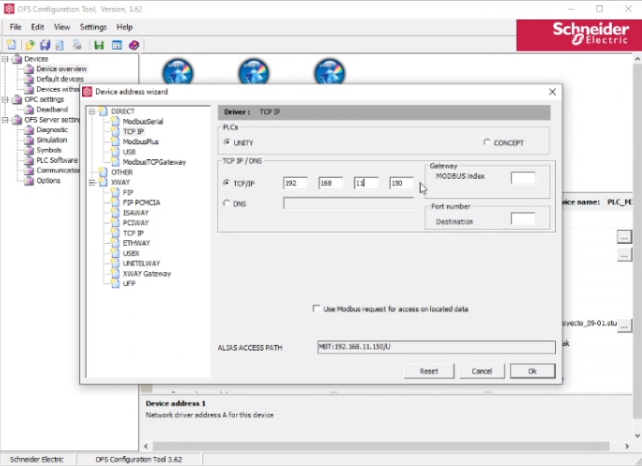
\includegraphics[width=70mm]{ofs1.png}}
	\subfigure[]{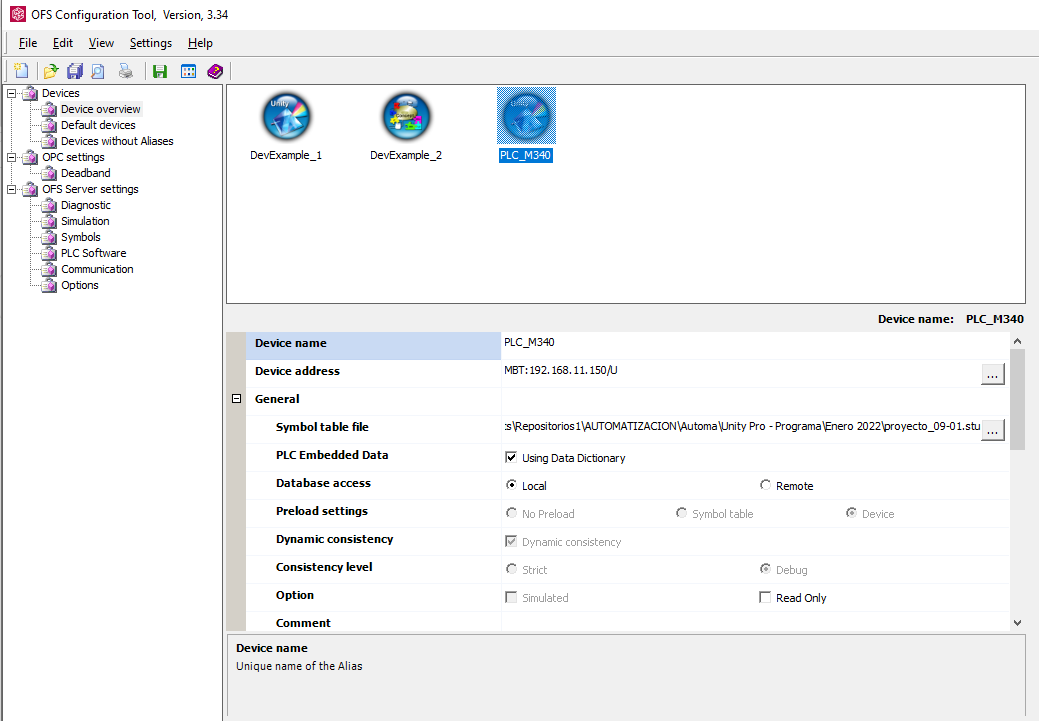
\includegraphics[width=70mm]{ofs2.png}}
	\caption{Configuración OPC} \label{fig:opc1}
\end{figure}


Una vez configurado el servidor se abre el programa \textbf{OPC Factory Server} dando inicio al servidor (Figura \ref{fig:opc2}a). Para observar si la comunicación esta establecida de forma correcta, se utilizó el programa \textbf{OFS Client} dónde se debió agregar el tag correspondiente a la variable a observar (Figura \ref{fig:opc2}b)

\begin{figure}[htbp]
	\centering
	\subfigure[OPC Factory Server]{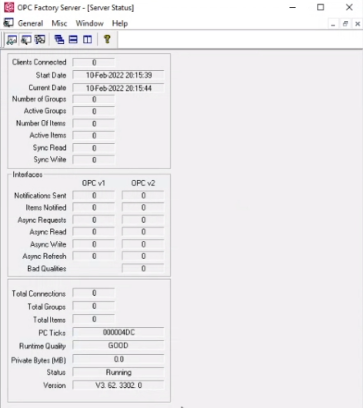
\includegraphics[width=40mm]{ofs3.png}}
	\subfigure[OFS Client]{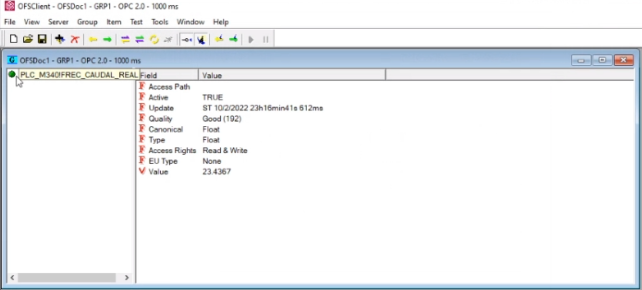
\includegraphics[width=80mm]{ofs4.png}}
	\caption{Conexión servidor OPC} \label{fig:opc2}
\end{figure}

Una vez corroborada la comunicación con el servidor OPC, se procedió a crear un cliente OPC en Simulink (perteneciente a Matlab) para adquirir y guardar las variables necesarias. 


\subsubsection{Uso de Matlab}
En el entorno Simulink se procedió a configurar un bloque de cliente OPC con la dirección IP donde se encuentra el servidor previamente creado. Luego, para leer las variables necesarias se creó un bloque de lectura OPC (Figura \ref{fig:opcsimu} a) y con un bloque \textit{Scope}, se activó la opción para que se guarden los vectores de las variables a estudiar (Figura \ref{fig:opcsimu} b). 


\begin{figure}[htbp]
	\centering
	\subfigure[]{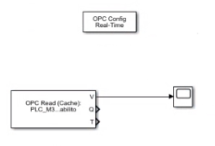
\includegraphics[width=40mm]{ofs5.png}}
	\subfigure[]{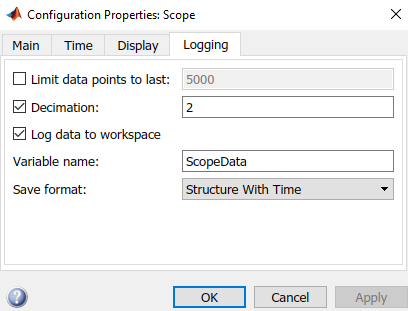
\includegraphics[width=60mm]{ofs6.png}}
	\caption{Cliente OPC en Simulink} \label{fig:opcsimu}
\end{figure}



\subsubsection{Estimación de la planta}